\documentclass[anonymous,12pt]{iopjournal}
\usepackage{amsmath,amssymb,amsthm,booktabs,array,microtype,graphicx,placeins}
\graphicspath{{figures/}}
\renewcommand{\topfraction}{0.9}
\renewcommand{\bottomfraction}{0.85}
\renewcommand{\textfraction}{0.09}
\renewcommand{\floatpagefraction}{0.8}
\hypersetup{hidelinks,pdftitle={Which material distributions can finite-aperture scattering data rule out?},pdfauthor={},pdfsubject={Electromagnetic inverse scattering}}
\fancyhead[L]{\small\sffamily Inverse Problems\quad Research paper}
\fancyhead[R]{\small Material bounds from finite-aperture data}
\newtheorem{theorem}{Theorem}[section]
\newtheorem{proposition}[theorem]{Proposition}
\newtheorem{corollary}[theorem]{Corollary}
\newcommand{\C}{\mathbb C}\newcommand{\R}{\mathbb R}
\newcommand{\Herm}{\operatorname{Re}_{H}}\newcommand{\Imag}{\operatorname{Im}_{H}}
\newcommand{\diag}{\operatorname{diag}}\newcommand{\tr}{\operatorname{tr}}
\newcommand{\Tail}{\mathcal T}\newcommand{\nn}{n_{-}}\newcommand{\np}{n_{+}}
\setlength{\headheight}{17pt}\setlength{\emergencystretch}{1.8em}
\numberwithin{equation}{section}
\setcounter{topnumber}{3}\setcounter{bottomnumber}{2}\renewcommand{\topfraction}{.94}\renewcommand{\textfraction}{.06}
\begin{document}
\noindent{\sffamily\small RESEARCH PAPER}\par\vspace{1.8ex}
\title{Which material distributions can finite-aperture scattering data rule out?}
\author{}
\begin{abstract}
A poor fit at one dielectric distribution gives little information about neighbouring distributions in a strongly scattering medium. We bound the distance from finite, noisy, multi-illumination measurements to the responses of every dielectric in a prescribed spatially varying interval. The shared local material equation gives a quadratic inequality on the illumination currents about an arbitrary background. At a specified error tolerance, an inertia count on a bordered matrix tests the entire interval, including when the current block is singular. Nested material hypotheses admit explicit transport of the spatial weights. On a 9,216-cell transverse-magnetic model, a disk of peak contrast 0.625 fits the data. On the same support, every member of a tapered class centred at peak four with nominal half-width 2.50 and a nonnegative lower cutoff misses the error ball. Its distance exceeds 1.72 times the radius with seven negative current modes. The verified width exceeds the usual norm-contraction cutoff by a factor of 5.14, and an admissible perturbation has spectral radius greater than one. The calculation also permits uncertainty at every background cell. On eight prospective targets the method eliminates 98 of 128 candidate boxes with no loss of a box containing the material; point-ranked full-wave refinement reaches a fit faster. Across 28 large-domain targets the data exclude every nonnegative first-Born fit, yet the Born image sometimes improves nonlinear initialization. These distinctions delimit what the measurements imply about a material class and about reconstruction.
\end{abstract}
\keywords{electromagnetic inverse scattering, finite aperture, contrast source, dielectric bounds, multiple illuminations, set inversion}
\section{Introduction}

A microwave inversion often returns several plausible images. At issue may be a particular physical claim: a strongly polarizable inclusion occupies this part of the specimen, with a specified allowance for variation within the inclusion and in its surroundings. A forward calculation tests one image. Ruling out the claim requires a bound valid for all images with those local allowances. This distinction matters when the total field inside an inclusion is very different from the incident field, and when a limited receiver aperture leaves a large space of currents unobserved.

Subspace methods separate visible and ambiguous currents and optimize the latter \cite{chen,zhong,ffttsom}. Contrast-source, new integral-equation and contraction integral-equation formulations couple those currents to a common material \cite{csi,nie,cie,chenbook}. Updating the propagation about an inhomogeneous background is classical in distorted-Born inversion \cite{dbim}. These methods supply reconstructions. We use the same background and receiver geometry to ask which entire classes of reconstructions remain possible. The observable is a lower bound in units of measured field, with an explicit error threshold. A region of material space can be excluded even when iterative recovery is poor.

The quadratic form of the field equations is well established in photonic design. Material duality, local conservation of power and their multi-excitation extensions bound responses under prescribed design restrictions \cite{angeris19,trivedi,angeris,moleskyglobal,moleskylocal,kuang,shim,miller}. Sector multipliers and integral quadratic constraints are standard tools for uncertain systems \cite{iqc,boyd,beck}. In the present inverse problem the complex port readings and the noise ball are fixed, and a scalar material at every cell is shared by all illuminations. A negative current subspace may change only a limited number of eigenvalues of the residual matrix. This pointwise rank restriction is lost if the lifted moments of many currents are averaged. The general matrix tools are inertia additivity, compression and eigenvalue interlacing \cite{haynsworth,tian,fan}. We identify the physical quadratic to which they apply for an arbitrary spatial interval and evaluate the resulting distance against a strong alternative.

Finite-measurement uniqueness and stability theorems ask whether data distinguish all coefficients under suitable prior restrictions \cite{alberti19,alberti21}. Monotonicity methods detect inclusions through an operator ordering with finitely many exceptional directions \cite{griesmaier_harrach,griesmaier_harrach_erratum,albicker}. Set inversion instead builds an enclosure of preimages of noisy data \cite{sivia}. Our calculation answers a user-specified membership question for the attainable \emph{data}, using the complete nonlinear scattering equations. It does not enumerate all feasible materials. Nonuniqueness can persist even for a small finite parameterization \cite{everett96,vasco}; a finite candidate list, whether produced by optimization or sampling, need not include the generating material.

We obtain three consequences from one current inequality. A test at the actual noise radius avoids tracking a spectrum through singular inverses. Exclusions can be inherited by nested intervals even when their midpoints move. With a common weak background, localized changes of interval endpoints require a matrix update whose order depends on the number of changed cells. Experiments ask separately whether the intervals can be distinguished beyond perturbative convergence, whether whole classes can be eliminated at useful cost, and whether the same tests improve a full-wave inversion. The third question requires comparison with a method that ranks individual samples by their exact scattered fields. Its answer differs from the first two.
\section{From local material intervals to a measured-field bound}\label{sec:theory}
\subsection{Physical model and reachable data}
Use $\exp(-{\rm i}\omega t)$, a real background wavenumber $k$, and the electric polarization invariant along the axis of a nonmagnetic cylinder. The scalar field obeys $(\Delta+k^2)E=-k^2\chi E$. The outgoing volume kernel is $k^2 {\rm i}H_0^{(1)}(k|x-y|)/4$ \cite{colton,richmond}. Its cell representation gives, for $n$ material cells, $s$ sources and $p$ receivers,
\begin{equation}
 E=B+GJ,\qquad J=XE,\qquad F(X)=SJ,\qquad X=\diag(\chi_i).
 \label{eq:vie}
\end{equation}
Here $B,J,E$ have $s$ columns and $S\in\C^{p\times n}$. A material is common to all sources. The $p\times s$ observed scattered field is $Y$. We work with the array and error scaling used to form that matrix; independent noises per optimized coherent source are not assumed. Data from any material in the admissible class $\mathcal B$ lie at a distance from $Y$ bounded below by
\begin{equation}
 \delta(\mathcal B;Y)=\inf_{X\in\mathcal B}\|SJ_X-Y\|_F.
 \label{eq:distance}
\end{equation}
For an error allowance $r$ a lower endpoint above $r$ rules out $\mathcal B$. Conversely, a single material in $\mathcal B$ with verified residual at most $r$ establishes compatibility. All physically admissible forward states are included if uniqueness of the forward equation is not assumed.

For a real interval at cell $i$ put $m_i=(u_i+\ell_i)/2$, $h_i=(u_i-\ell_i)/2$, $M=\diag(m_i)$, $D_h=\diag(h_i)$. Set $q=J-ME$. The scalar material equation gives $q_i=(\chi_i-m_i)e_i$ for the two row vectors. For real diagonal $W\succeq0,V=V^*$ put $A=D_h W D_h$. Then
\begin{equation}
 q^*Wq-E^*AE\preceq0,\qquad \Imag(q^*VE)=0 .
 \label{eq:row}
\end{equation}
Write $\Herm T=(T+T^*)/2$ and $\Imag T=(T-T^*)/(2{\rm i})$. The inequalities follow on multiplication by every coherent source vector. At one cell the two restrictions, with that row alone, recover the real material law in unlifted variables: testing vectors in $\ker e_i$ forces $q_i=z_i e_i$ (or $q_i=0$ if $e_i=0$), the equality makes $z_i$ real, and the inequality gives $|z_i|\le h_i$. Summing over cells is the source of relaxation.

When $I-GM$ is invertible let
\begin{align}
 E_c&=(I-GM)^{-1}B,\quad J_c=ME_c,\nonumber\\
 T&=(I-GM)^{-1}G,\quad P=S(I-MG)^{-1},\quad y=Y-SJ_c .
 \label{eq:shift}
\end{align}
Substitution in \eqref{eq:vie} gives $E=E_c+Tq$, $J=J_c+(I-MG)^{-1}q$, and $SJ-Y=Pq-y$. The order of $G$ and $M$ matters in the incident-field solve. An implementation can work in $J$ directly without inverting the background.

\begin{theorem}[Spatial contrast intervals]\label{th:main}
Set $D=(Pq-y)^*(Pq-y)$. Define
\begin{align}
 K&=P^*P+W-T^*AT+\Imag(VT),\\
 L&=P^*y+T^*AE_c+\tfrac{{\rm i}}{2}VE_c,\qquad C=y^*y-E_c^*AE_c,\\
 \mathcal A&=\begin{pmatrix}K&-L\\-L^*&C\end{pmatrix},\qquad
 P_s=\diag(0_n,I_s). \label{eq:border}
\end{align}
For any $t\ge0$ define $b(t)=[s-\nn(\mathcal A-tP_s)]_+$, where $\nn$ counts strictly negative eigenvalues. Every admissible residual matrix $D$ has at least $b(t)$ eigenvalues at least $t$. In particular
\begin{equation}
 \delta^2(\mathcal B;Y)\ \ge\ \int_0^\infty b(t)\,dt.
 \label{eq:count}
\end{equation}
If $\np(\mathcal A-tP_s)\ge n+j$ then the $j$th largest eigenvalue of $D$ is strictly greater than $t$. A single test therefore excludes $\mathcal B$ when $jt\ge r^2$. When $K$ is nonsingular, put $\nu=\nn(K)$ and $\mathcal H=C-L^*K^{-1}L$. The integral reduces to
\begin{equation}
 \Tail_\nu(\mathcal H)=\sum_{j=\nu+1}^{s}\big[\lambda_j^\downarrow(\mathcal H)\big]_+.
 \label{eq:tail}
\end{equation}
\end{theorem}
\begin{proof}
Adding the nonpositive sector and the zero optical form in \eqref{eq:row} to $D$ gives the quadratic lower matrix $[q;I]^*\mathcal A[q;I]$. The graph $a\mapsto(qa,a)$ is an injective map from $\C^s$. Restriction of a Hermitian form to its range cannot increase the negative index. At least $b(t)$ eigenvalues of $D-tI$ are therefore nonnegative. The span of the $n+j$ largest eigenvectors, with smallest eigenvalue $\gamma>0$, intersects the graph in dimension at least $j$. Since $\|(qa,a)\|\ge\|a\|$, the resulting lower gap $\gamma$ is uniform in $q$. Integrating the eigenvalue counting function and using $D\succeq0$ gives \eqref{eq:count}. Elimination of nonsingular $K$ gives a congruence of $\mathcal A-tP_s$ to $\diag(K,\mathcal H-tI)$ \cite{haynsworth}. Integrating its count yields \eqref{eq:tail}, including ties and $\nu\ge s$.
\end{proof}

At a singular $K$ the exact count has a useful source-space reduction. Let $Z$ span $\ker K$ orthonormally and let $Q$ be an orthonormal basis for $\ker(Z^*L)$. Set $a=\operatorname{rank}(Z^*L)$, $d_0=\dim\ker K-a$ and $H_r=Q^*(C-L^*K^\dagger L)Q$. Then
\[
 n_\pm(\mathcal A-tP_s)=n_\pm(K)+a+n_\pm(H_r-tI).
\]
Eliminate the range of $K$ and take a singular value decomposition of $Z^*L$. The $a$ nonzero singular values couple $a$ null-state coordinates to $a$ source coordinates. This saddle block has $a$ eigenvalues of each sign and a zero source--source block in its inverse. Eliminating it leaves $H_r-tI$ and $d_0$ uncoupled zeros. Hence \eqref{eq:count} equals $\Tail_{\nn(K)}(H_r)$ with $s-a$ source eigenvalues. In the strict positive-count implementation $\np(\mathcal A-tP_s)-n=\np(H_r-tI)-\nn(K)-d_0$. Exact common null directions can be removed before the test. At a mere numerical near-zero such removal requires an independent justification. The singular example in Appendix~\ref{app:tech} exhibits the difference.

In the original current coordinates put $U=I-MG$. The same augmented matrix has blocks
\begin{align}
 K_J&=S^*S+U^*WU-G^*AG+\Imag(VG),\\
 L_J&=S^*Y+U^*WMB+G^*AB+\tfrac{{\rm i}}2VB,\\
 C_J&=Y^*Y+B^*(MWM-A)B. \label{eq:unshifted}
\end{align}
Indeed $q=UJ-MB$. The congruence is block triangular with lower-right block $I_s$, so it preserves the threshold pencil's inertia and, if regular, the source Schur complement. These facts exclude an apparent gain from merely moving the origin of a fixed material hypothesis. The destructive term for a changed interval is quadratic in its true half-width. A fixed cell contributes none of this term; its known value still changes propagation. A strongly resonant background may make $T$ large even for small $h_i$.

\subsection{Nested hypotheses and the convergence radius}
The rows of the sector can be written as $\Herm[(j_i-\ell_i e_i)^*(j_i-u_i e_i)]$. For a fixed midpoint, widening the interval with fixed multipliers subtracts a positive semidefinite matrix from the bordered pencil. For changing midpoints there is a more useful weight rule.
\begin{proposition}[Transport under interval inclusion]\label{th:transport}
Let $I=[m-h,m+h]\subseteq I'=[m'-h',m'+h']$, with $0<h\le h'$. For arbitrary complex row vectors $(j,e)$ put $Q_I=(j-me)^*(j-me)-h^2 e^*e$. Then $(h'/h)Q_I-Q_{I'}\succeq0$. Thus any set of row weights for the parent box yields an equally strong or stronger count on the child by multiplying each sector weight by its own $h'_i/h_i$. Unchanged rows retain their weights. Known fixed cells may instead be eliminated exactly.
\end{proposition}
\begin{proof}
The coefficient matrix in $(j,e)$ has leading entry $\alpha-1$ and determinant
$-\alpha^2 h^2+\alpha(h^2+h'^2-(m-m')^2)-h'^2$. At $\alpha=h'/h$ this is $(h'/h)((h'-h)^2-(m-m')^2)\ge0$. When the chosen ratio $\alpha=h'/h$ equals one, interval inclusion and equal widths imply $I=I'$ and the difference vanishes. Sum the inequalities before performing any elimination. The common optical form in $J$ is unchanged. Eigenvalue ordering then proves the statement also for the direct threshold test.
\end{proof}
This elementary sector calculation permits a branch search to reuse evidence paid for on an ancestor. Taking an unchanged scalar weight on two nonconcentric intervals need not preserve the computed lower endpoint. Excluding an ancestor also excludes its descendants without any new linear algebra.

For width $w$ uniform on an active set with all other cells fixed, $\|wT\|_2<1$ on the active set suffices for a Neumann expansion of $(I-T\Delta)^{-1}$ for every $\|\Delta\|_2\le w$. This yields the comparison bound
\begin{equation}
 \delta\ \ge\ \Big[\|F(M)-Y\|_F-
      \|P\|_2\,w\|E_c\|_F/(1-w\|T\|_2)\Big]_+ .
 \label{eq:neumann}
\end{equation}
The operators in this formula are restricted to the active cells. A directional projection can sharpen the right side. Beyond this norm condition the series may still converge. For example a nilpotent perturbation can have arbitrarily large norm. Failure of the norm test also need not imply negative current inertia: at one cell with $T=2{\rm i},P=3,W=h=1,V=0$, $K=6>0$. To distinguish the mechanisms, we separately test $\rho(wT)$ for an admissible perturbation and count the negative directions of $K$. For nested $\mathcal B_w$, an excluded width and an admitted physical material at a larger width bracket $\inf\{w:\delta(\mathcal B_w;Y)\le r\}$ whenever the domain is regular and attainability is ensured, or bracket the corresponding first-witness width without that extra assumption.
\section{What can be decided before inversion?}\label{sec:use}
\subsection{Linear response, global contrast and losses}
The first Born port map is $A_B x=S\diag(x)B$. A port matrix $Z$ for which
$\Re\langle Z,A_B e_i\rangle_F\le0$ for every cell separates the nonnegative Born cone. Its distance from the measured field is at least $[\Re\langle Z,Y\rangle_F]_+/\|Z\|_F$. This test takes a single inner product after the signs have been checked for the array. Failure of this linear model justifies skipping a terminal Born fit. Nonlinear currents can fit the data for exactly the material whose Born prediction failed.

A second test applies Theorem~\ref{th:main} to $[0,u]^n$. It lower bounds the peak anywhere in the region without assigning a lower endpoint to any particular pixel. On an open two-dimensional domain the Hermitian part of the outgoing volume potential $H_G$ has positive principal symbol $k^2|\xi|^{-2}$. At fixed $k$, fixed bounded region $\Omega$ with boundary of area zero and fixed compact self-adjoint $C_0$, the negative-order Weyl law gives
$\nn(I-uH_G+C_0)\sim k^2|\Omega|u/(4\pi)$ as $u\to\infty$ \cite{ponge}. This describes a continuum spectral obstruction for that family of operators. Usable exterior angular orders instead scale roughly as $2ka$ for a region of circumscribed radius $a$ at fixed tolerance \cite{bucci87,bucci89}. Neither quantity fixes the distance to a measured field. The discrete index is bounded by $n$, and varying frequency, material classes or spatial weights changes the operator.

For a known loss tangent $\chi=(1+{\rm i}t_\ell)x$ with real $x$, translate by $M=(1+{\rm i}t_\ell)\diag(m_i)$. Apply \eqref{eq:row} to $q/(1+{\rm i}t_\ell)$ and $E$. In unrotated coordinates the optical equality is $\Imag(q^*VE)+t_\ell\Herm(q^*VE)=0$. The half-width in the complex plane is $|1+{\rm i}t_\ell|h_i$. For complex disks the modulus sector remains valid. A general rectangle needs its own valid constraints, and a passive lossy medium obeys a one-sided dissipative law. In particular a change about a lossy background can have negative imaginary part. A second, absolute-current inequality is available if $\Im\chi_i/|\chi_i|^2\ge\alpha>0$ on all nonzero cells. With $R=\Imag G$, $M_a=R+\alpha I\succ0$, $J_a=({\rm i}/2)M_a^{-1}B$ and $C_B=B^*M_a^{-1}B/4$, completing the square gives $(J-J_a)^*M_a(J-J_a)\preceq C_B$. Consequently the reachable receiver matrices lie in
\begin{equation}
 SJ_a+(SM_a^{-1}S^*)^{1/2} V_a C_B^{1/2},\qquad \|V_a\|_2\le1 .
 \label{eq:lossy}
\end{equation}
Indeed the least energy at fixed port value is given by the pseudoinverse on the range; the source Gram inequality is equivalent to a contraction \cite{douglas}. One can bound the distance to this set by its support function. These statements use only the declared losses. Real intervals, even signed ones, require no added absorption.

\subsection{A necessary current and an admissible search space}
For a third decision, suppose a real peak class can fit the data. In original coordinates write $V_-^*J=Z_-$, and let $\Lambda_-$ be the positive magnitudes of the negative eigenvalues of $K_J$. With nonsingular $K_J$ let $L_-=V_-^*L_J$ and $H_+=C_J-L_J^*K_{J,+}^\dagger L_J$. Minimizing only the positive square and testing on a source projector $Q$ yields, for $\|SJ-Y\|_F\le r$,
\begin{equation}
 \tr(QH_+)-r^2 \ \le\
 \|\Lambda_-\|_2\,\|Z_-\|_F^2+2\|L_- Q\|_F\|Z_-\|_F .
 \label{eq:norm}
\end{equation}
This gives a lower bound on the norm in the \emph{whole} negative space if the left side is positive. Individual modes need not have positive lower bounds. On six large-domain examples the necessary unweighted norm ranges from 7.65 to 22.00 for the cap one. Positive current that must accompany a chosen negative component can strengthen the estimate, but the improvement on the global material box was small. Appendix~\ref{app:limits} specifies the scope of that observation.

A solver's affine current space $J_d+UZ$ can be tested directly. Substitute it in \eqref{eq:unshifted} using
\[
 K_U=U^*K_JU,\quad L_U=U^*(L_J-K_JJ_d),\quad
 C_U=C_J+J_d^*K_JJ_d-2\Herm(J_d^*L_J).
\]
Theorem~\ref{th:main} holds on the stated space with $n$ replaced by its number of basis columns. Positive distances from this restricted test describe the proposed current space. A short basis alone cannot establish a positive distance for the full physical medium. The fourth decision concerns a complete spatial material neighbourhood, independently of the basis or where an optimizer starts. Excluding it can save a branch-constrained solve. Abandoning every future iterate of an unrestricted solver would additionally require that all those iterates stay in the excluded set.

For the contraction integral equation $\beta J=R(\chi)(\beta E+J)$, with $\beta>0$, $R(x)=\beta x/(\beta+x)$. On pole-free positive intervals,
$\beta j-R(\ell)(\beta e+j)=\beta^2(j-\ell e)/(\beta+\ell)$.
The sector built from both transformed endpoints is the original sector times the positive factor $\beta^4/[(\beta+\ell)(\beta+u)]$. This accounts for its invariance under consistent row reweighting. The inverse distance gives no universal rule for the optimizer's contraction parameter.

\begin{figure}[!htbp]\centering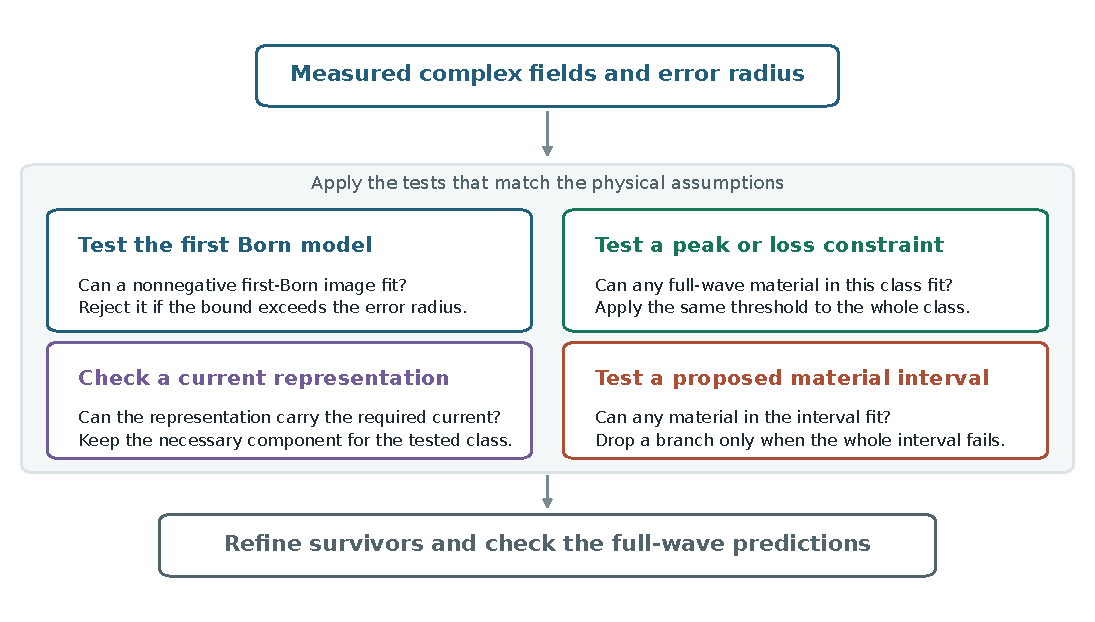
\includegraphics[width=.96\linewidth]{workflow.pdf}
\caption{Four physical decisions available before or alongside inversion. Only a full-wave check of a specified material establishes whether that material explains the observations.}\label{fig:workflow}
\end{figure}

\subsection{Sharing computation between spatial hypotheses}
A fixed array may receive new measurements for many specimens. Let $k_p$ cells change from the baseline interval $[0,b]$ to $[m_i-h_i,m_i+h_i]$ with weights $\alpha_i$ relative to the common sector weight $\mu$. In normalized current units each change adds, in the local rows $(j_i,e_i)$, the Hermitian form
\[
 D_i=\begin{pmatrix}\alpha_i-1&-(\alpha_i m_i-b/2)\\
 -(\alpha_i m_i-b/2)&\alpha_i(m_i^2-h_i^2)\end{pmatrix}.
\]
Thus the change of the \emph{bordered} form has rank at most $2k_p$ even when all $n$ background pixels are unknown. For a positive lower state block $K_b$, stack the pairs $(j_i,e_i)$ in pixel order as $T_p J+e_p$, with a zero in each incident current row and $B_i$ in its field row. Put $D_p=\mathrm{diag}_{\rm blocks}(D_i)$ in this order. In units consistent with $K_b$, let $J_b=K_b^{-1}L_b$, $Z_p=D_p^{-1}+T_pK_b^{-1}T_p^*$, $A_p=T_pJ_b+e_p$. If the inverses exist, completing the square gives
\begin{equation}
 \mathcal H'=\mathcal H_b+A_p^*Z_p^{-1}A_p,\qquad
 \nn(K')=\np(Z_p)-\np(D_p^{-1}) .
 \label{eq:update}
\end{equation}
For the second identity compare the two Schur complements of the matrix with diagonal $K_b,-D_p^{-1}$ and off-diagonal $T_p^*$. The source update follows from stationarity, including the constant $e_p^*D_pe_p$. A singular patch or state can be handled with the bordered count. Our implementation uses a one-sided Fourier floor on the \emph{base} state, then performs \eqref{eq:update} on this lower form; the count refers to that form. It computes the Gram of the patch rows once and retains only the receiver and source dependence in each subsequent test. Perturbative smallness near the high-contrast patch is unnecessary.

The initial geometry calculation includes the original-grid FFT or Green rows and their products. Dense branch algebra then costs order $(2k_p)^3$ per profile and order $(p+s)^2s+s^3$ per reading for the source form; forming the Gram can itself cost order $n k_p^2$ directly. The number and placement of patches are additional inputs. Without small changed supports or repeated geometry this offers no dimensional reduction. It also leaves the cost of discovering candidate material regions untouched.

\section{Experiments on finite-aperture scattering data}\label{sec:experiments}
\subsection{Materials, acquisitions and comparisons}
We count distinct simulated media and distinct laboratory objects. There are 72, plus a separate observation with two disjoint feasible material explanations. Table~\ref{tab:cohort} shows the role of each family. An acquisition at another frequency or with a different number of ports remains a paired observation. Previously examined objects are identified as such. The eight prospective pool targets were first generated after the weights, comparison arms, stopping rules and metrics were fixed. A ground-truth contrast or material mask was never used to rank a proposed region, select a reconstruction, or verify a lower bound. Declared supports in the compact tests are shared priors. The full-domain tests allow 9,216 independent parameters. Some contracts intentionally use identical forward and inverse grids to isolate an algebraic mechanism. Such a contract provides no continuum error estimate.

\begin{table}[!htbp]\centering\small
\caption{Distinct specimens contributing to each question. Array sizes are transmitters by receivers. These specimens contribute 120 registered acquisition views. A six-parameter ambiguity observation brings the total to 121. Two additional low-amplitude site controls reuse registered geometries.}\label{tab:cohort}
\begin{tabular}{@{}p{.33\linewidth}rp{.48\linewidth}@{}}\toprule
Material family & Number & Measurement and role\\\midrule
Large-domain, real & $6+22$ & $96^2$, $ka=11.85$, $10\times20$, 10\%. Six also at $32\times32$, 2\%.\\
Compact annular targets & 7 & $24^2$, $ka=4.27$, $12\times48$; cap 5 and data routing.\\
Loss-tangent geometries & 4 & $ka=3.55,7.40$, $10\times20$; three paired loss angles, 2\%.\\
Weak to moderate controls & $2+4$ & Two earlier shapes and four new shapes, first Born and full-wave data.\\
Chamber targets & $3+4$ & Fresnel at 4, 6, 8 GHz; Manitoba at seven frequencies from 3 to 6 GHz.\\
Structured sample pools & $4+8$ & Development and prospective samples respectively; $24^2$, $4\times16$, half aperture, 1.25\%.\\
Learned flow on its own geometry & 3 & $32^2$, signed contrast, two opposing sources, 16 receivers; 1\% tolerance.\\
Other mechanism controls & 5 & One $24^2$ annulus, one $32^2$ shape, one low-contrast disk, two site controls.\\\bottomrule
\end{tabular}
\end{table}

The large-domain synthetic measurements have physical frequency 400 MHz and a $2\,{\rm m}\times2\,{\rm m}$ field of view, with fixed total incident fluence within a paired comparison. The errors are joint complex Frobenius radii. We report a downward field-distance endpoint $d/r$ and, where available, a feasible point's upward endpoint. For inversion we report relative material $\ell^2$, target and background errors and held-out complex fields. Each comparator sees the same observations, geometry, masks and allowable material inputs within a comparison. The candidate-pool optimizer enforces its box throughout. The subsequent CIE comparison uses the actual contraction integral equation with its own state variables. Timings include proposals, full-wave solves, verification and unsuccessful attempts at the specified stage. Results on freshly simulated and previously archived measurements are distinguished.

\begin{figure}[!htbp]\centering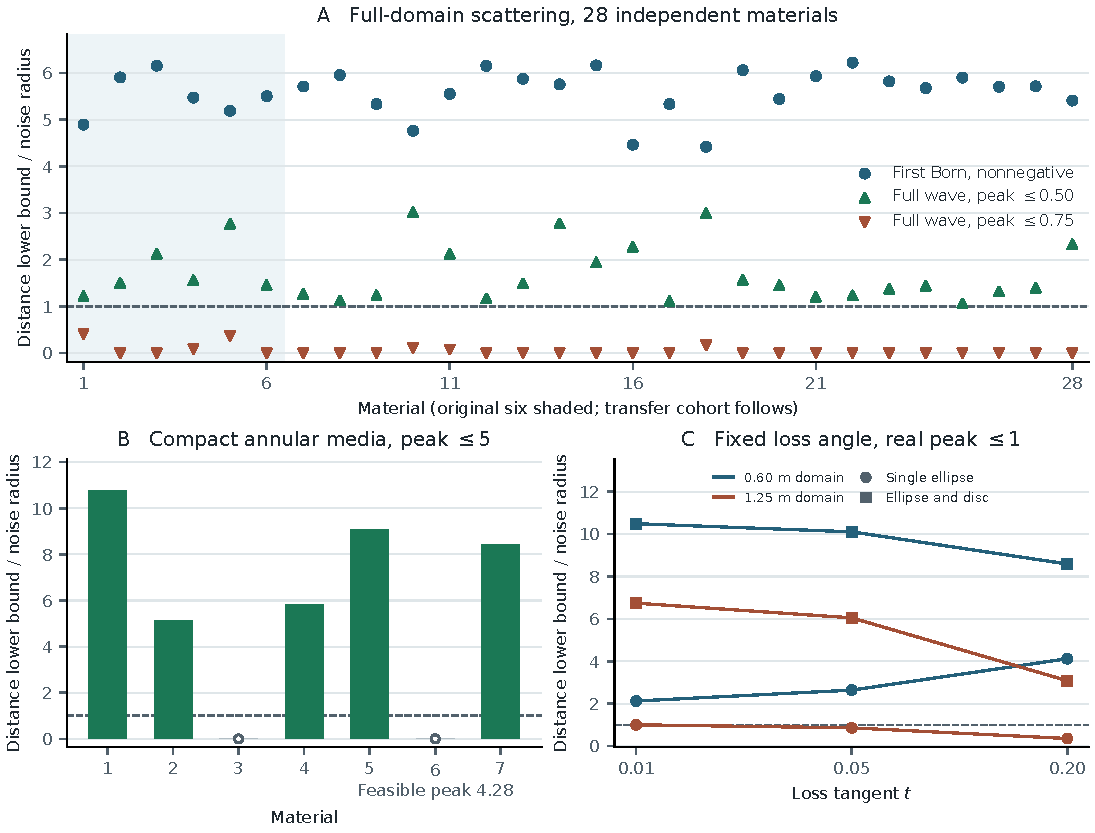
\includegraphics[width=.98\linewidth]{benchmark.pdf}
\caption{Bounds across every member of the primary lossless family and two other physical regimes. The reference line is the measurement error radius. Loss-angle comparisons use the same complex-material contract at each abscissa. Frequencies, hypotheses and noise levels are never counted as additional specimens.}\label{fig:benchmark}
\end{figure}

\subsection{From a blind contrast cap to a strong material neighbourhood}
On the primary 28 large-domain targets the nonnegative Born cone misses the receiver matrix by at least 43.88--61.94\% of its norm. At 10\% noise all 28 rule out the \emph{nonlinear} cap 0.50, with distances from $1.062r$ to $3.019r$. The same test at 0.75 excludes none. At 2\% noise with 32 sources and 32 receivers the six detailed cases give respectively five, three and one exclusions at 0.78125, 0.8125 and 0.84375, and none at one. Thus the strongest global statement on this six-target array remains that at least one cell of one target exceeds 0.84375. On seven distinct compact annular examples five exclude a cap of five. An admitted member of one of the other examples has peak 4.282. The difference in electrical area, illumination and measurement radius matters in comparing these regimes.

We next prescribe a high-valued material neighbourhood. Its circular support is fixed in each test, and its centre is either set by geometry or placed using only a Born adjoint of the readings. Contrast varies independently from cell to cell across an interval around a tapered profile. Vacuum outside the support gives an exact restriction of \eqref{eq:vie} to its active cells; all original ports remain. Table~\ref{tab:native} distinguishes a matched positive quadratic, a weaker material restriction and a physical point. A high-contrast class can be impossible for the simple reason that its support is wrong. On the first two 96² strong targets the lower endpoints removed at fixed support still give exclusions. On the 32² test that change instead leaves the comparison undecided. Two further experiments placed a known 78-cell dielectric of contrast 3.25 outside 437 uncertain cells, with the remaining 8,701 exterior cells fixed at vacuum. Including all interactions with this host gives lower bounds $29.00r$ and $27.73r$ under identity weighting, both with $\nu=7$ and 32 illuminations.

\begin{table}[!htbp]\centering\small
\caption{Same observations and supports, with nominal peak four. Columns show strict lower endpoints rounded down. The positive comparison is the best verified choice shown on the identical box; the final column relaxes the lower endpoints or supplies an admitted point. The asterisk marks an obstruction for the scalar spatial weights specified below.}\label{tab:native}
\begin{tabular}{lrrrrrp{.23\linewidth}}\toprule
Grid, object & Cells & $w$ & $\nu/s$ & $d/r$ & Pos. & Same support\\\midrule
$24^2$, annular & 177 & 2 & 2/12 & 57.37 & 54.74 & relaxed $>56.14r$\\
$32^2$, independent & 89 & 2 & 9/10 & 10.70 & 12.23 & relaxed $>0.43r$\\
$96^2$, slotted block & 749 & 2 & 9/32 & 18.94 & 25.05 & relaxed $>3.34r$\\
$96^2$, second target & 749 & 2 & 9/32 & 21.98 & 23.20 & relaxed $>6.27r$\\
$96^2$, disk & 1153 & 2.5 & 7/32 & 1.728 & $*$ & low peak fits within $0.99995r$\\\bottomrule
\end{tabular}
\end{table}

The disk provides a separation on \emph{one and the same support}. Its peak-0.625 reference satisfies the full-wave data within $0.999950r$. For the high branch the nominal peak is four; at the profile maximum the allowed interval is $[1.5,6.5]$. The strict lower endpoint is $1.7284581r$. A receiver-null unit vector has sector value at most $-0.22201567$ and radiation at most $1.4740\,10^{-17}$. It prevents positivity for every positive scalar sector multiplier with identity spatial weight and zero optical multiplier. For the recorded normalization the same conclusion holds for absolute optical-to-sector multiplier ratios below $1.5062\,10^{16}$. This is a limitation of those weights; general spatial reweighting is allowed by the theory.

For a tapered nominal profile $c_i$ the tested endpoints are $\max(0,c_i-w)$ and $c_i+w$. Thus $w$ is the nominal half-width; clipping acts only at the lower boundary. In this disk the norm contraction limit is bracketed by $[0.48604895,0.48604902]$. For the homogeneous upper perturbation in the box, $|\tr((wT)^4)|/1153>1.3932$ and hence $\rho(wT)>1.0864$. This makes the distinction stronger than failure of a sufficient contraction condition. The measured exclusion extends at least $5.1435$ times as far as its norm cutoff. At width $3.86436632$ the same low-peak physical witness belongs to the expanded box. The first possible fit is bracketed between $2.50$ (up to one binary rounding unit) and this latter width; its exact location is unknown. The proposal scan took 124.48 s wall and 125.04 s CPU across 241 boxes. The 22 main high-precision endpoint checks took 396.71 s wall and 583.71 s CPU. The extra radius and radiation analysis for the disk cost roughly 138 CPU s in addition to the high-box check. In particular this direct verification on a large support is a substantial additional calculation.

\begin{figure}[!htbp]\centering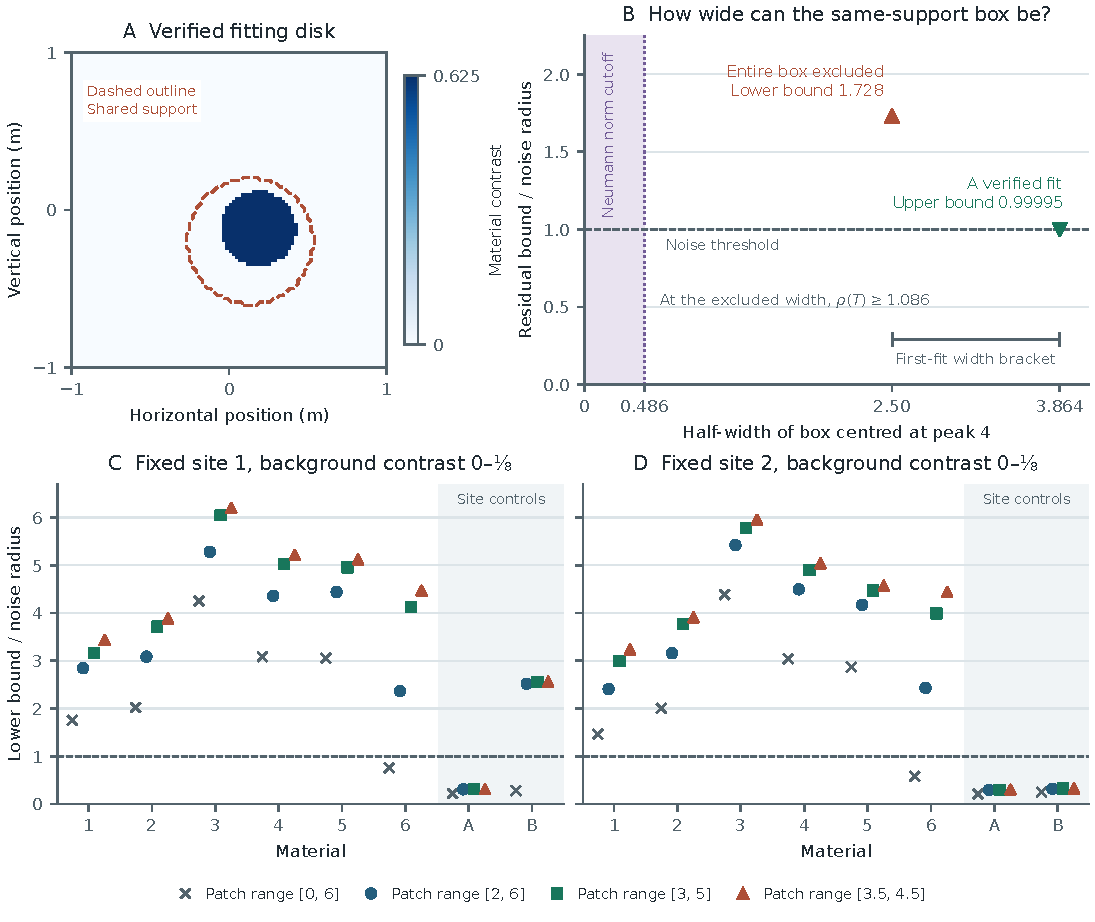
\includegraphics[width=.98\linewidth]{branches.pdf}
\caption{A high-contrast branch can be ruled out on a support that admits a different material. Allowing uncertainty in the entire exterior weakens the conclusion. The two-site comparison uses $8\times8$ candidate patches and the same array for eight receiver matrices.}\label{fig:branches}
\end{figure}

We relaxed the support assumption on the same 96² array. Two sites were specified in advance, each with $8\times8$ cells and independently variable contrasts. The other 9,152 cells now have arbitrary contrast in $[0,b]$. With nominal patch $[2,6]$ and $b=1/16$, both site hypotheses are excluded for each of the six detailed targets, with attained lower endpoints at least $7.89r$. Two additional compact controls of peaks 3.884 and 4.470 lie in their own site hypotheses, and the opposite site can be excluded in both. Doubling the background allowance to $1/8$ leaves only three of the six exclusions on both sites for the original matched weights. Transporting the parent $[0,6]$ weights using Proposition~\ref{th:transport} recovers all six at both sites, with lower endpoints from $2.36r$ to $5.42r$. This improves on directly reusing the broad-parent decision: the parent leaves one of the six unresolved on each site. For the two controls the wrong site is now excluded in one case ($d/r$ approximately 2.518), while the other is unresolved (approximately 0.496); both correct sites are retained. These endpoints use the better of two prespecified base multipliers $2^{-12}$ and $2^{-10}$. To isolate the role of the high lower endpoint, we generated a paired peak-0.625 amplitude on each of the same two patches. Both belong to the broad parent and fit their own readings within $0.999951r$. For these particular data the shifted $[2,6]$ child remains undecided even after weight transport: at $b=1/8$ the attained endpoints are $0.242r$ and $0.277r$. The comparison establishes an improvement across the six readings and exposes a remaining class of same-site ambiguities of the lower-bound test. The two new amplitudes are paired controls in addition to the registered acquisition views. Geometry work took $0.97+2.70+3.46$ s. The 32 original profiles and 256 readouts took 16.44 s including all choices. The transported comparison, repeating geometry and evaluating 24 profiles for eight readings each, took 17.27 s wall.

\subsection{What does a candidate pool buy?}
On four development objects a fixed data-driven proposal constructs sixteen overlapping boxes and four samples per box. All candidates share the same known $7\times7$ support on a $24^2$ physical grid; multi-source scattering within it is exact. The distinct objects have peaks from 3.99 to 4.60. The fit uses four illuminations and 16 of 32 receivers; disjoint receiver and illumination readings are reserved for scoring. For each box the same full-wave bound-constrained quasi-Newton solver can vary all 49 active materials for 42 function evaluations. The strong point comparator pays for full-wave propagation of all 64 samples, then refines boxes in order of point residual until the first verified fit. The exhaustive comparator refines all sixteen. Geometric support and unrestricted reciprocal current transfer can fit any of the measured port matrices on this patch (Appendix~\ref{app:tech}); material information is essential.

Conventional and source-directional Neumann bounds rule out four of 64 boxes. Replacing all positive lower endpoints by zero permits the sector computation to reject fourteen. The centred intervals eliminate forty, leaving respectively nine, six, five and four candidates. All eight boxes that actually cover their generating material survive. These eight are broad proposal priors; no narrow box in this development set covers its generator. Selecting only the best single sample misses a noise-ball fit on three of four objects. Refining in order of point fit instead reaches the tolerance after one or two boxes on every object. The complete interval procedure uses 1,154 optimization factorizations against 2,367 for exhaustive refinement, yet wall time rises from 0.082--0.111 s to 0.777--1.135 s per object. Point ranking followed by refinement takes 0.028--0.036 s. Exclusion of every member of a box and receipt of a single acceptable image have different costs.

To reduce that cost we used the bordered count at just one source threshold. On the four development objects it recovers all forty exclusions with at most two scalar weights. Before generating eight new target geometries, the weights, threshold, refinement allowance, sixteen proposal families and noise rule were fixed. Figure~\ref{fig:pools} shows all eight outcomes. Respectively 13, 12, 13, 12, 9, 14, 13 and 12 boxes were excluded. All ten truth-containing boxes survived. Every exclusion was independently enclosed by complex ball arithmetic. Seven objects yielded a verified physical fit with all three methods. On the remaining object the generator fits the noisy measurement, but the constrained optimizations exhausted their budgets. An unresolved or unvisited box was never classified as a physical branch.

\begin{table}[!htbp]\centering\small
\caption{Prospective 49-cell inversions, eight independent materials. Medians are per target. The fixed input error is 1.25\%. Receiver and illumination holdouts are scored independently. All three methods had seven accepted endpoints; the common failure is included in the error medians.}\label{tab:pool}
\setlength{\tabcolsep}{3pt}\begin{tabular}{@{}lrrrrr@{}}\toprule
Method & Wall (ms) & CPU (ms) & LU & Image & Rx / Tx\\\midrule
All sixteen boxes & 82.5 & 81.9 & 535.5 & 10.02\% & 1.16 / 1.67\%\\
Points until first fit & 37.1 & 37.0 & 183 & 10.02\% & 1.16 / 1.67\%\\
Test surviving boxes & 54.6 & 54.5 & 179.5 & 10.02\% & 1.16 / 1.67\%\\
\bottomrule\end{tabular}
\end{table}
The point-ranked arm stops after one or two boxes on seven targets. On the eighth, all sixteen fail to reach tolerance (74.6 ms and 577 LU). The bordered arm refines all two to seven survivors per target. On the eighth this takes 56.8 ms and 119 LU. On every target its best material comes from the broad initial prior box. The median independent interval replay took a further 362.7 ms per target and rechecked the 98 exclusion decisions. Table~\ref{tab:pool} includes the online floating-point error bounds and the endpoint forward checks. Including the additional replay gives roughly 0.42 s per object. Solver setup, proposals, ranking, field solves and endpoint checks were timed on the same Apple M4; rates need not carry over to another implementation.

To isolate the cost of a single image, we then gave both arms exactly the same stopping objective on these eight exposed targets. Both propagate all 64 points, refine the best sample of each ranked box, and stop at the first verified fit. One arm also screens boxes before refinement. In ten paired runs per target, both return identical materials on all eight; both find seven fits. Summing the eight per-target median times yields 0.258 s without screening and 0.296 s with screening. The latter uses 1,409 instead of 1,803 full-wave factorizations. All seven successful targets take longer when screened. On the common failure it skips fourteen boxes, reducing time from 57.65 to 34.61 ms and factorizations from 577 to 183. An independent replay of the 98 exclusions cost a further 2.137 s for the eight targets. Thus fewer field solves yield a time saving on the hard target, but not on this cohort overall.

\begin{figure}[!htbp]\centering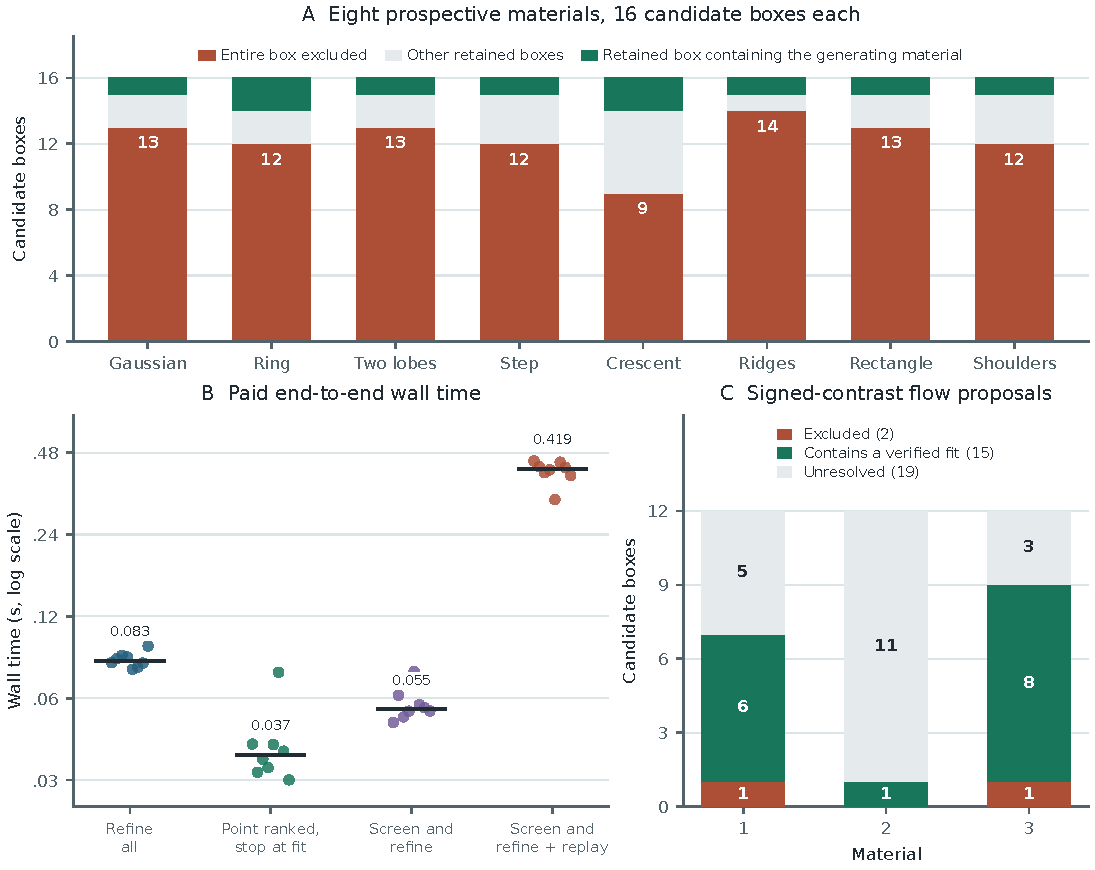
\includegraphics[width=.99\linewidth]{pools.pdf}
\caption{What is gained by testing whole material boxes? Paired prospective results show the number excluded and the time to an image. A separate learned generator uses its own signed material and aperture convention. Its boxes can contain physically feasible alternatives while missing the generating material.}\label{fig:pools}
\end{figure}

\paragraph{Same four comparisons with a current-domain inversion.}
We repeated the branch experiment using a hard-box contraction integral equation. All four arms use the same deterministic visible current, rank four, Fourier current updates at 4, 16 and 36 columns, two contraction parameters, a common source-wise conjugate-gradient update, and a shared contrast at each active cell. The contrast is projected into the proposed interval at every voxel readout. Settings were fixed before these current iterations; the twelve geometries had already been used in the preceding comparisons. The pure CIE schedule leaves \emph{all} twelve outside the discrepancy radius (best per case $1.668r$--$4.307r$). Although the box test avoids many iterations, this experiment alone does not demonstrate faster recovery.

We therefore followed each current-domain output by the same 42-evaluation box-constrained nonlinear corrector, with original-field acceptance. Table~\ref{tab:ciepool} includes the new calculation for all 12 objects. Every arm now gives a verified fit on every object. The interval arm returns the same materials as exhaustive refinement in each case. The online time falls from 4.96 s to 1.89 s. Including the independent 2.882 s ball-arithmetic replay of all 138 exclusions brings this to 4.775 s, close to the exhaustive 4.963 s. All eighteen truth-containing boxes survive. The more demanding comparison is the point-ranked arm, which stops at a fit and takes 0.89 s. The choice between eliminating material classes and returning a first compatible map remains observable even with a genuine current-space inversion and successful endpoints.
\begin{table}[!htbp]\centering\small
\caption{Paired, independently timed current-domain refinement followed by a physical corrector on 12 targets already exposed to the study. Wall and LU counts are totals. Image and withheld-port errors are reported in the text as medians. All 48 selected images fit their measurement balls. Independent ball-arithmetic replay adds 2.882 s to the bordered arm.}\label{tab:ciepool}
\begin{tabular}{@{}lrrrr@{}}\toprule
Material selection & Wall, s & CPU, s & Full-wave LU & Fits\\\midrule
All boxes & 4.963 & 4.878 & 8672 & 12/12\\
Point rank until fit & 0.890 & 0.873 & 2430 & 12/12\\
Neumann survivors & 6.456 & 6.331 & 8464 & 12/12\\
Bordered-test survivors & 1.892 & 1.866 & 3516 & 12/12\\\bottomrule
\end{tabular}
\end{table}
The interval arm has median material error 6.71\%, held-out receiver error 0.978\% and held-out illumination error 1.407\%. Point ranking yields 6.42\%, 1.108\% and 1.370\%. At the 42-evaluation allowance, direct point-ranked physical optimization without CIE missed one object ($1.042r$). In a follow-up restricted to that exposed failure, doubling the direct allowance yields a verified $0.9531r$ at the second ranked box in 0.041--0.042 s. The CIE and corrector point arm on that object used 0.071 s. This check removes the apparent necessity of the CIE start. No target was replaced after the initial failure.

A learned flow was evaluated on its original $32^2$ signed-contrast model with two opposing incident waves and 16 observed receivers. We regenerated 64 samples per object using the stored weights, formed twelve Ward clusters and expanded each coordinate range by 0.10. This experiment uses three previously exposed held-out materials and clean archived readings with a 1\% tolerance. Their generating materials are outside \emph{all} 36 boxes. After 39 budgeted full-wave evaluations per cluster, verified physical materials enter six, one and eight boxes respectively. Best point residuals are $0.276r$, $0.937r$, $0.470r$, with material errors 26.35, 79.36 and 51.53\% despite held-out receiver errors below 1\%. The signed sector excludes two further boxes at $3.294r$ and $8.455r$, both with positive state curvature and perturbation norm at most 0.52. The standard Neumann distance and tested directional bounds reject neither. Across the three readings, fifteen boxes admit verified physical points, two are excluded and nineteen remain unresolved. Across two objects, 25 pairs of disjoint boxes contain verified alternatives. The original generating materials were independently accepted in their own data balls. Verified lower bounds for the diameter of the material feasible set are 26.35, 79.36 and 51.53\% of the respective generating norms. The sector search and verification here take about 34 s for the three readings, including about 13 s for the 36 proposals and 21.36 s for independent ball-arithmetic checks and their shared setup. Point ranking to the first fit reaches cluster ranks one, seven and one, with stage-summed totals of 7.21, 11.91 and 4.55 s. The corresponding box-first totals are 29.87, 21.50 and 27.72 s; exhaustive refinement takes 19.37, 17.50 and 17.01 s. An observation with two much more widely separated materials at an extremely small tolerance gives a useful counterexample to always selecting one branch: Appendix~\ref{app:tech} reports both directly checked physical endpoints.

Figure~\ref{fig:maps} shows the selected fields on a common contrast scale. The low residual in the last row is consistent with the observed receiver matrix even when the image visibly differs from the generating material.
\begin{figure}[!htbp]\centering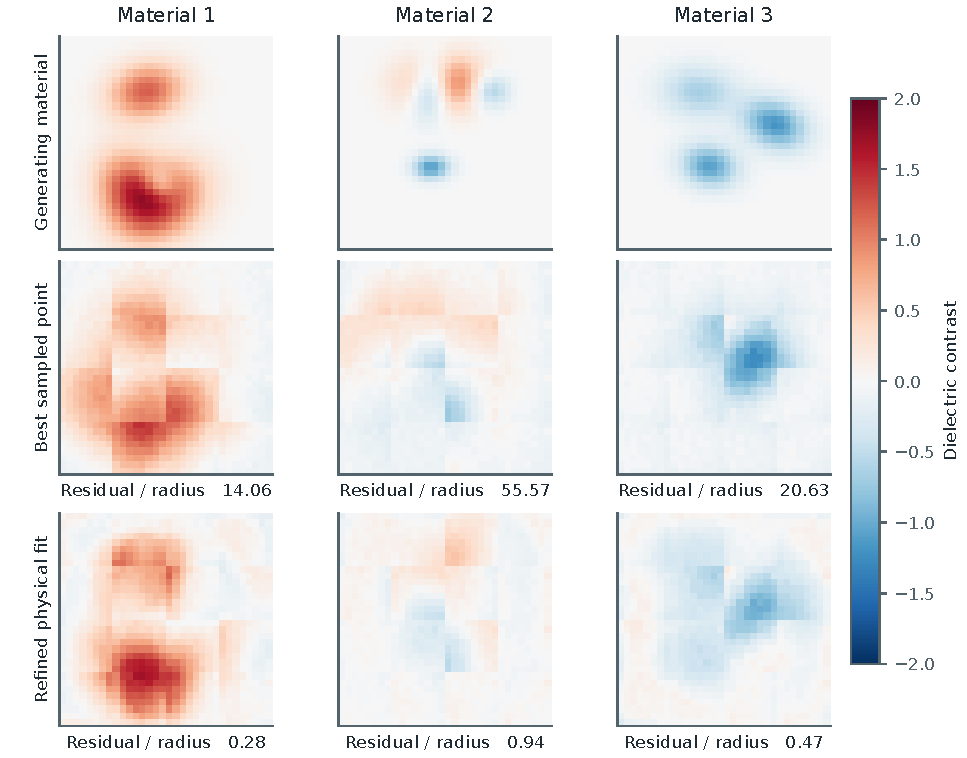
\includegraphics[width=.83\linewidth]{material-alternatives.pdf}
\caption{Three signed-contrast materials and alternatives proposed from two incident waves. Middle row: the best of 64 original samples by full-wave data misfit. Bottom row: the best full-wave fit from the twelve refined material boxes. Selection uses the measured receiver data alone; the top row is revealed for scoring.}\label{fig:maps}
\end{figure}

\subsection{Does the decision improve nonlinear reconstruction?}
On the 28 primary targets, the Born decision took a median 0.142 ms after 0.269 s of geometry preparation. Its rejected images still supply useful initial guesses. With the same $[0,4]$ box, 24² grouped material updates on the native forward grid and sixteen objective evaluations, Born initialization improves the training residual on 15 of 28 targets and the material error on ten. One example changes from $9.825r$ to $4.662r$ and from 0.996 to 0.870 in relative material error. No endpoint in either arm on these targets attains the error radius. A routed zero initialization costs 106.61 s summed over the 28 objects, versus 108.15 s with a Born start. On four new weak-to-moderate geometries Born initialization improves all four final material and residual errors, although two fail the linear terminal test. The test detects a physical failure of the linear model; it does not select an optimal solver.

Matching the material box in a native contraction integral-equation method gives 32.30 and 32.72 s for 28 vacuum and Born starts. At 16 current steps the median material errors are 0.913 and 0.919, inside-target errors 0.686 and 0.682, background RMS 0.674 and 0.686, held-out field errors 1.100 and 1.107. Independent full-wave residuals are $10.46r$ and $10.61r$. Two longer three-stage runs still ended above $8r$ after 96 steps. These are capped optimization comparisons. They do not establish a lower bound on the performance of a converged CIE or SOM solve.

On the slotted block and staggered grooves at 2\% noise, the 13-dimensional negative current projection must have norm above 15.76 and 19.76 respectively for any fit at peak at most one. The ordinary 100-column Fourier basis already meets this space at principal angles of $0.91$--$5.47$ degrees. We replace thirteen columns by orthogonalized negative modes at fixed basis width, measured aperture, deterministic-current rank, and iteration count. Relative image errors improve from 0.959 to 0.922 and 0.819 to 0.779, but training residuals worsen from $59.66r$ to $60.45r$ and $53.31r$ to $53.80r$; held-out complex fields worsen on both. The necessary norm is met by all four peak-clipped points, whose field discrepancies exceed $65r$. Directly pulling back the bordered inequality to the actual affine subspaces also rules out neither basis. A fixed contraction parameter of two accounts for much of the early reduction obtained by a peak-informed choice. A larger necessary norm supplies no quantitative independent gain in image recovery in these comparisons.

Finally, two full-domain CIE iterates were tested with actual local boxes. With half-width 0.04 both the new and perturbative bounds were undecided. Narrowing to 0.005 gave $7.970r$ and $17.952r$; the analogous Neumann bounds already gave $5.599r$ and $16.353r$. All restart policies chose the same continuation. Ordinary unconfined continuation left the two narrow boxes in respectively 94 and 140 pixels. This directly checks the premise needed for interpreting a local box as a basin. The box proof added 0.67--0.79 s.

\subsection{What changes with losses and laboratory measurements?}
On four distinct positive loss-tangent geometries, with $t_\ell=0.01,0.05,0.20$ paired within each, all twelve known-phase Born cones can be excluded. The compact example at $t_\ell=0.05,u=0.75$ illustrates what dissipation contributes under the same physical assumptions. Every common scalar energy multiplier gives less than $0.80975r$; applying the same law with separate weights in coherent source directions gives more than $1.01323r$, and the full receiver ellipsoid more than $1.02003r$. At $u=1.25$ one compact example gains from jointly using the absolute material sector and the dissipative information in distinct illumination directions. The larger examples can remain inside the relaxed receiver ellipsoid. Their undetermined peaks cannot be assigned the bound from a different loss tangent.

Real measurements from the Fresnel and Manitoba facilities \cite{fresnel,manitoba} delimit the error interpretation. Born distances exceed the reported reference error scales in three of nine and 25 of 28 frequency views respectively. No Fresnel view at cap 0.5 clears the held-out empty-scene scale. At passive cap one, the large Manitoba nylon cylinder at 3 GHz leaves 4.018\% of the field norm for further loaded-scene error after accounting for calibration spread. In separate training-only Born fits, relative receiver holdout errors range from 80.2 to 97.9\% at Fresnel and from 68.1 to 107.9\% at Manitoba; separate source holdout errors are 91.4--116.8\% and 69.0--104.8\%. A loaded-scene forward error below the quoted headroom has not been established. The chamber data therefore support a conditional error budget and an independent field prediction comparison.

\section{Discussion}

The distinction between a peak hypothesis and a branch hypothesis is observable in the same experiment. Data exhausted the attainable bound on a blind contrast cap near 0.84 in a large domain. Yet a spatial class with peak between 1.5 and 6.5 could be rejected on the same type of array, even though the permitted variation extended well beyond convergence of a background perturbation series. The additional information is the explicit set of spatial alternatives. Each exclusion is conditional on its support, box widths, constitutive law, ports and error allowance. Declaring the complement of a proposed inclusion weak can provide much of the information. A comparison against the identical support with its lower endpoints removed is therefore indispensable.

A small number of negative propagating-current directions has a specific use. It limits the number of source combinations which an unobserved current can cancel simultaneously. It places no comparable bound on the number of unknown pixels, candidate branches or local minima. Born inconsistency, a lower bound on the peak and a necessary norm in a mode subspace each answer different physical questions. They can identify an impossible terminal state or an invalid restriction. They supply little evidence that a particular initialization, Fourier truncation or continuation step will finish sooner.

The remaining practical issue is how the candidate intervals are obtained. Structured priors gave informative boxes at modest cost on known compact support. Particles from a learned flow on its own geometry gave boxes that omitted the exact generating distributions and still admitted widely different materials within the data tolerance. A collection of overlapping boxes has no automatic posterior coverage, probability interpretation or claim to exhaustive topology. In particular, survival of only one proposed box would not establish unique recovery. Nor can a local exclusion justify abandoning an unconstrained optimization trajectory that can move outside it.

Transfer to a continuum or to a laboratory would require a common upper bound on the modelling error for the whole candidate class. A held-out empty-chamber calibration measures only part of that error. The most directly supported use is to test a specified material claim on a calibrated finite array before investing in all of its reconstructions. For a user who needs only one compatible image, the point-ranked alternative is sufficiently inexpensive that the broader answer currently costs extra.
\appendix
\section{Checking the field and spectrum endpoints}\label{app:tech}
The finite cell model uses the equal-area disk self term \cite{richmond}. For square cells of side $h$, set $z=kh/\sqrt\pi$. The Green entries away from the diagonal are $\mathrm i\pi zJ_1(z) H_0^{(1)}(k d)/2$ at centre-to-centre distance $d$. The diagonal is $\mathrm i\pi z H_1^{(1)}(z)/2-1$. A port outside the region uses the off-diagonal rule. We retain the incident field, complex datum normalization and Green representation supplied with each array. In the main large-domain comparison the bound applies to the exact represented padded Fourier symbol and the original receiver and illumination coefficients. Known exterior pixels can be eliminated through the corresponding block system. For example, with known contrast $M_h$ and perturbations only on the selected cells $T_c$, the active-field equation is obtained by applying $T_c^*(I-GM_h)^{-1}$ to $B+G T_cq_c$. This accounts for every interaction with the fixed host. No coarse eigenvectors are taken as a complete fine-grid basis.

An interval matrix is evaluated by midpoint--radius arithmetic with outward rounding \cite{arb}. To count a whole nonsingular state spectrum we use an approximate frame $V$ as a proposal, verify $\lambda_{\min}(V^*V)>0$, and enclose $V^*KV$ by signed, separated intervals or a one-sided complement estimate. For the direct test at $t$ it is enough to exhibit $n+j$ independent columns with positive restricted form. On the prospective small boxes a binary64 calculation bounds complex dot-product, assembly, frame and residual errors before an online decision. Each positive result was also replayed directly by evaluating Gram products of the proposed columns in ball arithmetic at the original endpoints. This second computation avoids assumptions about the proposing eigensolver. Candidate forward solves are upper endpoints; a small observed floating residual alone cannot justify an exclusion or inclusion. In the signed $32^2$ experiment a full-state residual and a verified inverse-defect bound enclose the forward response. No positivity of the material was used.

A rational singular example checks the counting convention. In excess-current coordinates take one active cell, $h=W=1,V=0,T=5/4$, two sources, $E_c=(3/4,0)$, and two receivers with $P=(3/4,0)^\top$, $y=\diag(-5/4,2)$. Then $K=L=0$, $C=\diag(1,4)$. The count integral is five and the admissible contrast perturbation $-1$ attains squared residual five. Here $\mathcal A-tP_s=\diag(0,1-t,4-t)$. The uncompressed strict count $\np\ge1+j$ can detect only $j=1$ and $t<1$. Removing the exact common null state restores the full two-source spectrum in the integrated count. This is an algebraic control for a persistent zero. The large radiating examples use a resolved numerical spectrum.

For the full-domain branch calculation write the baseline quadratic at $[0,b]$ in units of its positive sector multiplier. The uncompressed state is $I-b\Herm G+S^*S/\mu$. A finite subset of a Fourier convolution is a compression of its padded embedding, so this operator is bounded below by $(1-b\max\Re\widehat G)I+S^*S/\mu$. When the scalar floor is positive, its inverse is computable by a receiver-size system. We keep the exact simultaneous linear and constant terms of the original base quadratic. After replacing the state block by this lower block, local changes to the endpoint rows have exactly the form \eqref{eq:update}. Arb Fourier inversion encloses the required submatrix of $G$, the two row Grams, all sources and receiver products, and the state and source eigenvalue bounds. For each patch the reduced inertia is checked on all $2k_p$ coordinates, and the positive tail is rounded down using a near-unitary frame and its verified defect. Unknown background pixels have entered the calculation before this reduction. A positive base floor is an explicit sufficient condition for this implementation.

The conventional perturbation comparison uses the same background, active coordinates and endpoints. In the disk example let $T$ denote the exact active Green operator about the candidate material. Interval linear solves bound the two-norm from below and above. An upper perturbation $wI$ respecting the box gives $n\rho(wT)^4\ge|\tr((wT)^4)|$ by the complex eigenvalue trace identity; it does not require normality. When floating construction of tabulated material endpoints rounds inward, the proof for an ideal real interval uses its largest guaranteed contained width. This accounts for less than $4.5\,10^{-16}$ at the quoted disk width.

In the structured 49-cell problem, put $U=[S^\top,B]$. We verified a left inverse $LU=I$ for the corresponding joint field frame in both the structured-pool support comparison and the separate applicable flow geometry. For any complex matrix $Y$, $T_0=L^\top\bigl(\begin{smallmatrix}0&Y\\Y^\top&0\end{smallmatrix}\bigr)L$ is symmetric and has $ST_0B=Y$. Thus support and unbounded reciprocity alone admit every measured matrix on these arrays. Such a $T_0$ need not be produced by a passive diagonal material. It is the missing constitutive information that the sector supplies.

A six-cell example checks how a sound branch test handles actual ambiguity. We reused two known numerical materials and an existing three-illumination, single-receiver measurement, without repeating the root search. Independent 128-bit evaluations of the original full-wave equations bound their residuals by $1.603\,10^{-15}$ and $1.415\,10^{-15}$, compared with $r=2^{-30}\|Y\|_F>7.6340\,10^{-11}$. Their RMS material separation exceeds 1.15879. Disjoint real boxes of half-width 0.05 around their respective centres must both survive. This proves compatibility of distinct materials with the declared observation ball. It does not assign algebraic multiplicity to the rounded central reading.

\section{Scope of the blind-box comparison}\label{app:limits}
For nonsingular $K$ diagonalize its negative and positive parts and write a physical displacement as $J-J_0=Nc+Pv$ in energy-normalized bases, with $J_0=K^{-1}L$. Then $D\succeq\mathcal H+v^*v-c^*c$. Individual material rows require
\[
 [(I-XG)P]_i v=[X(B+GJ_0)-J_0]_i-[(I-XG)N]_i c .
\]
The nonzero source-dependent term must be retained. If these rows imply $v^*v+M_Y\succeq c^*\Pi c$ on the whole tested box for an orthogonal projection of rank $c_0$, only $\nu-c_0$ unconstrained coordinates remain. Interlacing gives $\Tail_{\nu-c_0}(\mathcal H-M_Y)$ as a lower bound. For the fixed 13-mode state form on the six $96^2$ arrays, a verified upper estimate on the attainable gain of separately weighted rows rules out every selection of at most 59 cells as a route to a cap-one exclusion, including the tested signed centre charges. This is a limit on that local-row construction. It neither constructs a low-peak material nor bounds methods that exploit a different material hypothesis. Equations \eqref{eq:row} and \eqref{eq:border} change all of the relevant rows when a new spatial interval is specified, which is why the two results are consistent.

In the large-domain study, contrast and total incident fluence are held fixed when varying the number of sources. Measurements can add angular information until the port fields repeat combinations within tolerance. On a half aperture the restrictions of passivity and optical power can constrain receiver-invisible currents that still radiate. On a dense full ring the corresponding remaining modes can radiate extremely weakly. Their finite number across sources, rather than a large positive optical eigenvalue, can still strengthen a distance estimate. Neither mechanism makes spatial recovery unique. At a single voxel $G={\rm i}$, $S=B=1$, the midpoint of $J(0)$ and $J(1)$ would require complex contrast $2/5+{\rm i}/5$. Even a scalar real material interval can have a nonconvex set of full-wave responses.

\section*{Data availability}
The finite operators, observation identifiers, decision arrays, comparison timings, and scripts used for the figures are supplied with the research data. The two laboratory data sources are described in \cite{fresnel,manitoba}. Identifying repository links are provided separately for anonymous review.
\section*{Acknowledgments}
OpenAI Codex assisted with mathematical analysis, numerical experiments and preparation of the manuscript. Google Gemini assisted with independent analysis and review. The authors take responsibility for the content.
\begin{thebibliography}{99}
\bibitem{chen} Chen X 2010 Subspace-based optimization method for solving inverse-scattering problems \emph{IEEE Trans. Geosci. Remote Sens.} \href{https://doi.org/10.1109/TGRS.2009.2025122}{\textbf{48} 42--49}
\bibitem{zhong} Zhong Y and Chen X 2009 Twofold subspace-based optimization method for solving inverse scattering problems \emph{Inverse Problems} \href{https://doi.org/10.1088/0266-5611/25/8/085003}{\textbf{25} 085003}
\bibitem{ffttsom} Zhong Y and Chen X 2011 An FFT twofold subspace-based optimization method for solving electromagnetic inverse scattering problems \emph{IEEE Trans. Antennas Propag.} \href{https://doi.org/10.1109/TAP.2010.2103027}{\textbf{59} 914--927}
\bibitem{csi} van den Berg P M and Kleinman R E 1997 A contrast source inversion method \emph{Inverse Problems} \href{https://doi.org/10.1088/0266-5611/13/6/013}{\textbf{13} 1607--1620}
\bibitem{nie} Zhong Y, Lambert M, Lesselier D and Chen X 2016 A new integral equation method to solve highly nonlinear inverse scattering problems \emph{IEEE Trans. Antennas Propag.} \href{https://doi.org/10.1109/TAP.2016.2535492}{\textbf{64} 1788--1799}
\bibitem{cie} Zhong Y and Xu K 2019 Contraction integral equation for three-dimensional electromagnetic inverse scattering problems \emph{J. Imaging} \href{https://doi.org/10.3390/jimaging5020027}{\textbf{5} 27}
\bibitem{chenbook} Chen X 2018 \emph{Computational Methods for Electromagnetic Inverse Scattering} (Singapore: Wiley) \href{https://doi.org/10.1002/9781119311997}{doi:10.1002/9781119311997}
\bibitem{dbim} Chew W C and Wang Y M 1990 Reconstruction of two-dimensional permittivity distribution using the distorted Born iterative method \emph{IEEE Trans. Med. Imaging} \href{https://doi.org/10.1109/42.56334}{\textbf{9} 218--225}
\bibitem{angeris19} Angeris G, Vu\v{c}kovi\'{c} J and Boyd S P 2019 Computational bounds for photonic design \emph{ACS Photonics} \href{https://doi.org/10.1021/acsphotonics.9b00154}{\textbf{6} 1232--1239}
\bibitem{trivedi} Trivedi R, Angeris G, Su L, Boyd S, Fan S and Vu\v{c}kovi\'{c} J 2020 Bounds for scattering from absorptionless electromagnetic structures \emph{Phys. Rev. Applied} \href{https://doi.org/10.1103/PhysRevApplied.14.014025}{\textbf{14} 014025}
\bibitem{angeris} Angeris G, Vu\v{c}kovi\'{c} J and Boyd S 2021 Heuristic methods and performance bounds for photonic design \emph{Opt. Express} \href{https://doi.org/10.1364/OE.415052}{\textbf{29} 2827--2854}
\bibitem{moleskyglobal} Molesky S, Chao P, Jin W and Rodriguez A W 2020 Global $\mathbb{T}$ operator bounds on electromagnetic scattering: upper bounds on far-field cross sections \emph{Phys. Rev. Research} \href{https://doi.org/10.1103/PhysRevResearch.2.033172}{\textbf{2} 033172}
\bibitem{moleskylocal} Molesky S, Chao P and Rodriguez A W 2020 Hierarchical mean-field $\mathbb{T}$ operator bounds on electromagnetic scattering: upper bounds on near-field radiative Purcell enhancement \emph{Phys. Rev. Research} \href{https://doi.org/10.1103/PhysRevResearch.2.043398}{\textbf{2} 043398}
\bibitem{kuang} Kuang Z and Miller O D 2020 Computational bounds to light--matter interactions via local conservation laws \emph{Phys. Rev. Lett.} \href{https://doi.org/10.1103/PhysRevLett.125.263607}{\textbf{125} 263607}
\bibitem{shim} Shim H, Kuang Z, Lin Z and Miller O D 2024 Fundamental limits to multi-functional and tunable nanophotonic response \emph{Nanophotonics} \href{https://doi.org/10.1515/nanoph-2023-0630}{\textbf{13} 2107--2116}
\bibitem{miller} Miller O D, Polimeridis A G, Reid M T H, Hsu C W, DeLacy B G, Joannopoulos J D, Solja\v{c}i\'{c} M and Johnson S G 2016 Fundamental limits to optical response in absorptive systems \emph{Opt. Express} \href{https://doi.org/10.1364/OE.24.003329}{\textbf{24} 3329--3364}
\bibitem{iqc} Megretski A and Rantzer A 1997 System analysis via integral quadratic constraints \emph{IEEE Trans. Autom. Control} \href{https://doi.org/10.1109/9.587335}{\textbf{42} 819--830}
\bibitem{boyd} Boyd S and Vandenberghe L 2004 \emph{Convex Optimization} (Cambridge: Cambridge University Press) \href{https://doi.org/10.1017/CBO9780511804441}{doi:10.1017/CBO9780511804441}
\bibitem{beck} Beck A and Eldar Y C 2006 Strong duality in nonconvex quadratic optimization with two quadratic constraints \emph{SIAM J. Optim.} \href{https://doi.org/10.1137/050644471}{\textbf{17} 844--860}
\bibitem{haynsworth} Haynsworth E V 1968 Determination of the inertia of a partitioned Hermitian matrix \emph{Linear Algebra Appl.} \href{https://doi.org/10.1016/0024-3795(68)90050-5}{\textbf{1} 73--81}
\bibitem{tian} Tian Y 2013 Closed-form formulas for calculating the extremal ranks and inertias of a quadratic matrix-valued function and their applications \href{https://arxiv.org/abs/1301.2567v1}{arXiv:1301.2567v1}, Corollary~4.5, equation~(4.38)
\bibitem{fan} Fan K 1949 On a theorem of Weyl concerning eigenvalues of linear transformations I \emph{Proc. Natl Acad. Sci. USA} \href{https://doi.org/10.1073/pnas.35.11.652}{\textbf{35} 652--655}
\bibitem{alberti19}Alberti G S and Santacesaria M 2019 Calder\'on's inverse problem with a finite number of measurements \emph{Forum Math. Sigma} \href{https://doi.org/10.1017/fms.2019.31}{\textbf{7} e35}
\bibitem{alberti21}Alberti G S and Santacesaria M 2022 Infinite-dimensional inverse problems with finite measurements \emph{Arch. Ration. Mech. Anal.} \href{https://doi.org/10.1007/s00205-021-01718-4}{\textbf{243} 1--31}
\bibitem{griesmaier_harrach}Griesmaier R and Harrach B 2018 Monotonicity in inverse medium scattering on unbounded domains \emph{SIAM J. Appl. Math.} \href{https://doi.org/10.1137/18M1171679}{\textbf{78} 2533--57}
\bibitem{griesmaier_harrach_erratum}Griesmaier R and Harrach B 2021 Erratum: monotonicity in inverse medium scattering on unbounded domains \emph{SIAM J. Appl. Math.} \href{https://doi.org/10.1137/21M1399221}{\textbf{81} 1332--37}
\bibitem{albicker} Albicker A and Griesmaier R 2023 Monotonicity in inverse scattering for Maxwell's equations \emph{Inverse Probl. Imaging} \href{https://doi.org/10.3934/ipi.2022032}{\textbf{17} 68--105}
\bibitem{sivia}Jaulin L and Walter E 1993 Set inversion via interval analysis for nonlinear bounded-error estimation \emph{Automatica} \href{https://doi.org/10.1016/0005-1098(93)90106-4}{\textbf{29} 1053--64}
\bibitem{everett96}Everett M E 1996 Homotopy, polynomial equations, gross boundary data, and small Helmholtz systems \emph{J. Comput. Phys.} \href{https://doi.org/10.1006/jcph.1996.0070}{\textbf{124} 431--41}
\bibitem{vasco}Vasco D W 2000 An algebraic formulation of geophysical inverse problems \emph{Geophys. J. Int.} \href{https://doi.org/10.1046/j.1365-246x.2000.00188.x}{\textbf{142} 970--90}
\bibitem{colton} Colton D and Kress R 2019 \emph{Inverse Acoustic and Electromagnetic Scattering Theory} 4th edn (Cham: Springer) \href{https://doi.org/10.1007/978-3-030-30351-8}{doi:10.1007/978-3-030-30351-8}
\bibitem{richmond} Richmond J H 1965 Scattering by a dielectric cylinder of arbitrary cross section shape \emph{IEEE Trans. Antennas Propag.} \href{https://doi.org/10.1109/TAP.1965.1138427}{\textbf{13} 334--341}
\bibitem{ponge} Ponge R 2023 Connes\textquoteright{} integration and Weyl\textquoteright{}s laws \emph{J. Noncommut. Geom.} \href{https://doi.org/10.4171/JNCG/509}{\textbf{17} 719--767}
\bibitem{bucci87} Bucci O M and Franceschetti G 1987 On the spatial bandwidth of scattered fields \emph{IEEE Trans. Antennas Propag.} \href{https://doi.org/10.1109/TAP.1987.1144024}{\textbf{35} 1445--1455}
\bibitem{bucci89} Bucci O M and Franceschetti G 1989 On the degrees of freedom of scattered fields \emph{IEEE Trans. Antennas Propag.} \href{https://doi.org/10.1109/8.29386}{\textbf{37} 918--926}
\bibitem{douglas} Douglas R G 1966 On majorization, factorization, and range inclusion of operators on Hilbert space \emph{Proc. Amer. Math. Soc.} \href{https://doi.org/10.1090/S0002-9939-1966-0203464-1}{\textbf{17} 413--415}
\bibitem{fresnel} Geffrin J-M, Sabouroux P and Eyraud C 2005 Free space experimental scattering database continuation: experimental set-up and measurement precision \emph{Inverse Problems} \href{https://doi.org/10.1088/0266-5611/21/6/S09}{\textbf{21} S117--S130}
\bibitem{manitoba} Gilmore C, Zakaria A, Mojabi P, Ostadrahimi M, Pistorius S and Lo Vetri J 2011 The University of Manitoba microwave imaging repository: a two-dimensional microwave scattering database for testing inversion and calibration algorithms \emph{IEEE Antennas Propag. Mag.} \href{https://doi.org/10.1109/MAP.2011.6138442}{\textbf{53} 126--133}
\bibitem{arb} Johansson F 2017 Arb: efficient arbitrary-precision midpoint-radius interval arithmetic \emph{IEEE Trans. Comput.} \href{https://doi.org/10.1109/TC.2017.2690633}{\textbf{66} 1281--1292}
\end{thebibliography}

\end{document}
